% !TeX root = ../main.tex

\appendix{B}{視覺化神經纖維分析工具}
\label{app:tool}

AEL 雖為全自動流程，於臨床導入時仍有兩項實務需求：

\begin{enumerate}
  \item \textbf{中介產物之視覺檢驗：}最終指標為一純量計數 $N_{\text{pred}}$，其品質高度依賴前處理、成本圖與多源擴張等中介結果之合理性。
  \item \textbf{人為修整之回饋迴圈：}於染色嚴重斷裂或微粒標註有誤之切片上，自動重建結果未必符合專家判讀。
\end{enumerate}

本研究為此實作一套桌面端圖形介面工具（以下簡稱\textbf{本工具}），以 Electron 框架~\cite{electron2026}建構，前端負責圖層疊合與互動式編輯，第~\ref{chap:method}~章之 AEL 則以 Python 實作為後端運算核心。本附錄摘要其介面組成與操作邏輯，並詳述與第~\ref{chap:method}~章直接相關之參數與輸出格式。

\section{介面布局}
\label{sec:tool-layout}

主視窗分為四大區塊（圖~\ref{fig:tool-layout}）：\textbf{左側邊欄}依功能分為檔案、圖層、演算法與纖維四個分頁，集中全部控制項；\textbf{頂部工具列}含互動模式切換與清除按鈕；\textbf{中央畫布}為影像圖層與重建圖之疊合區，支援拖曳平移與以游標為中心之滾輪縮放，載入新樣本時自動適配視野；\textbf{底部狀態列}顯示唯讀統計（第~\ref{sec:tool-statusbar}~節）。

\begin{figure}[htbp]
  \centering
  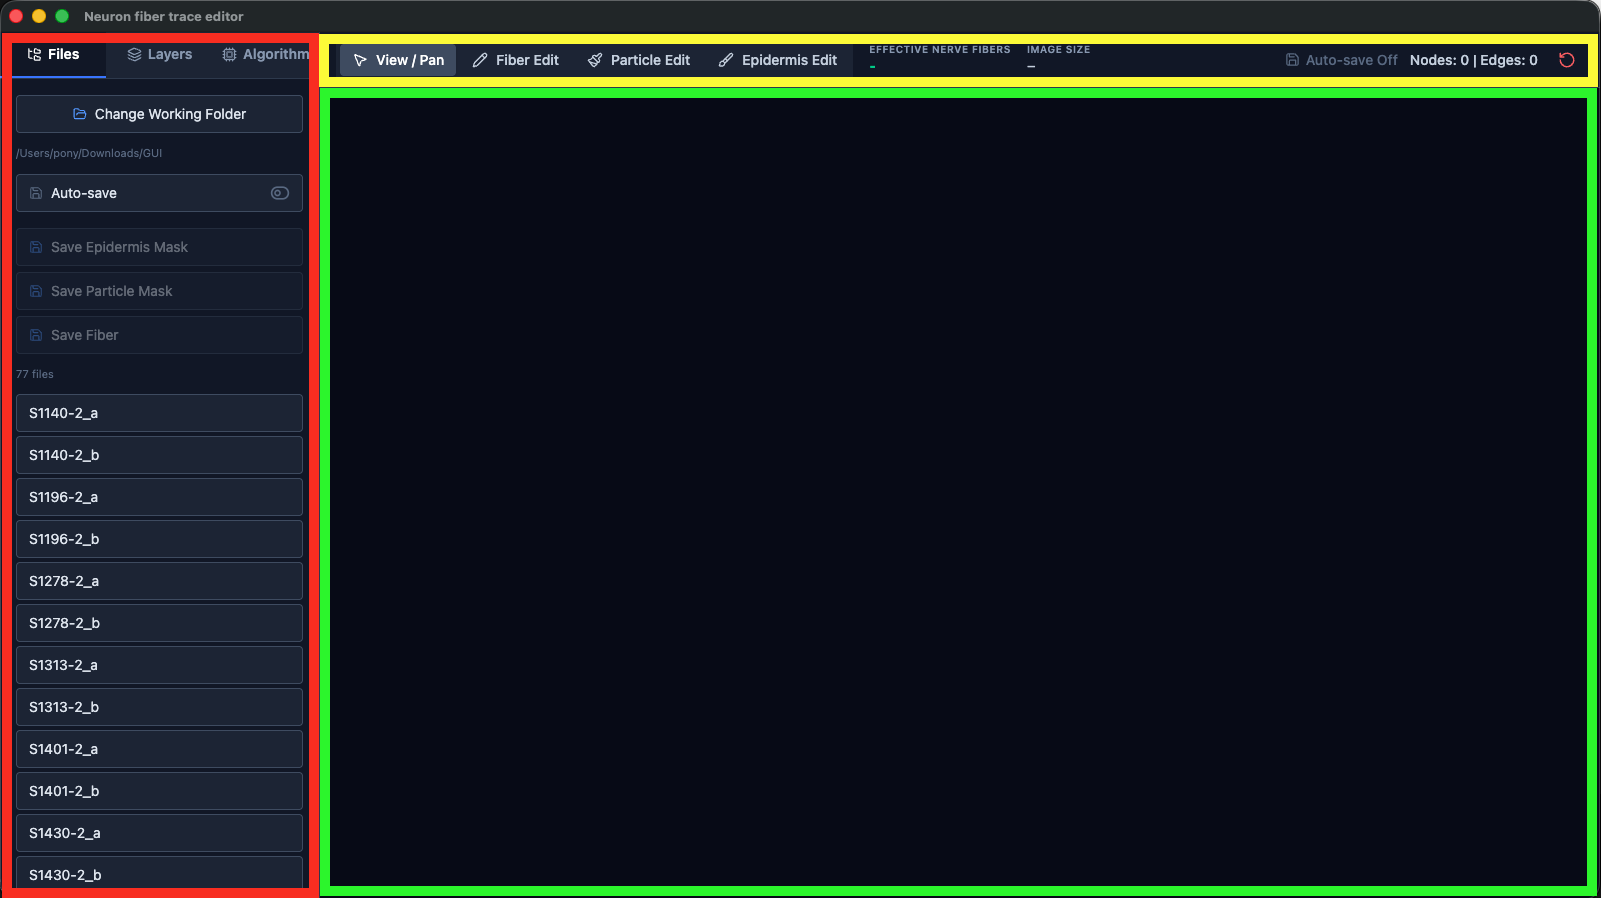
\includegraphics[width=0.85\linewidth]{figures/gui/main.png}
  \caption[本工具主視窗布局]{本工具主視窗布局。圖中紅色框（左側）為左側邊欄、黃色框（上方）為頂部工具列、綠色框（中央）為中央畫布（影像與重建圖之疊合區）、橘色框（下方）為底部狀態列。}
  \label{fig:tool-layout}
\end{figure}

\section{側邊欄分頁}
\label{sec:tool-sidebar}

\paragraph{檔案分頁：}指定資料來源並集中全部儲存控制（第~\ref{sec:tool-io}~節）。使用者選定一工作目錄，其下每個子資料夾視為一個樣本，預設內含原始影像（\texttt{image}）、表皮遮罩（\texttt{epidermis}）與纖維微粒遮罩（\texttt{particle}）三張影像。點選清單中任一樣本即自動載入該三層，毋需逐張上傳；若該樣本先前已有自動儲存之工作階段，其圖層設定、重建圖與計數結果亦一併還原。

\paragraph{圖層分頁：}畫布上最多疊合五張影像圖層與一層重建圖，由下而上依序為原始影像、表皮遮罩、感興趣區域遮罩 $M_{\text{ROI}}$、前處理結果圖（Sato 響應圖 $I_{\text{enhanced}}$）、纖維微粒遮罩與重建圖，本分頁提供各層之顯示切換與透明度控制。原始影像可選擇顯色通道，預設為綠色通道，亦即 AEL 後端實際使用之輸入；其餘四層皆為\textbf{灰階圖層}，以影像亮度作為透明度、再覆蓋使用者選定之純色，故響應或標註愈強之像素愈接近飽和、背景則保持透明。重建圖之節點依\textbf{度數} (degree) 上色，以區分端點（度數 $1$）、分支點（度數 $3$ 以上）與中繼點；邊則以\textbf{綠色}標示經計數判定之\textbf{有效跨越段}（即第~\ref{sec:crossing}~節 $N_{\text{pred}}$ 之構成）、其餘為藍色。邊若含後端回傳之像素層軌跡，即以折線沿該軌跡繪製以呈現多源區域擴張所回溯之實際路徑，手動新增者則為直線。

\paragraph{演算法分頁：}為 AEL 之三階段控制面板，依序為\textbf{感興趣區域}（第~\ref{subsec:roi}~節，得 $M_{\text{ROI}}$）、\textbf{前處理}（第~\ref{subsec:enhance}~節之增強鏈，並同步計算像素成本圖 $C$）與\textbf{重建}（第~\ref{sec:dijkstra}~節至第~\ref{sec:skeleton}~節，輸出 $G_{\text{trim}}$）；各階段須前一階段完成後方能啟用，另有一鍵串接三階段之\textbf{全部執行}按鈕。重建之執行會\textbf{完整覆蓋}既有重建圖，前次之手動編輯不予保留。參數設定視窗共九項可調參數，與第~\ref{chap:method}~章之對應符號列於表~\ref{tab:params-all}；更動即時生效並保存於本機，惟\textbf{不會自動觸發重算}。其中 \texttt{Min Particle Number} 為第~\ref{subsec:coverage-filter}~節之微粒涵蓋門檻 $N_{\min}$，本研究預設為 $0$（即不啟用該檢查），留予使用者逐切片調整之彈性。

\begin{table}[htbp]
  \centering
  \caption{參數設定視窗之全部參數列表（依區段分組）。}
  \label{tab:params-all}
  \small
  \setlength{\tabcolsep}{4pt}
  \begin{tabular}{p{2.4cm}lccp{2.6cm}}
    \toprule
    區段 & 參數名稱 & 預設值 & 對應符號 & 來源 \\
    \midrule
    \multirow{6}{2.4cm}{前處理\\(Preprocessing)}
       & \texttt{Epidermis Offset (px)}    & $50$   & $\text{offset}$    & 式~\eqref{eq:roi} \\
       & \texttt{Background Removal Radius} & $2$    & $r_{\text{bg}}$    & 式~\eqref{eq:tophat} \\
       & \texttt{CLAHE Clip Limit}         & $40$   & $\beta$            & 式~\eqref{eq:clahe} \\
       & \texttt{CLAHE Grid Size}          & $768$  & $n_{\text{tile}}$  & 式~\eqref{eq:clahe} \\
       & \texttt{Sato $\sigma$ Start}      & $1$    & $\sigma_{\min}$    & 式~\eqref{eq:sato} \\
       & \texttt{Sato $\sigma$ Stop}       & $3$    & $\sigma_{\max}$    & 式~\eqref{eq:sato} \\
    \midrule
    連結\newline(Pathfinding) & \texttt{Prune Threshold} & $20.0$ & $\tau$ & 第~\ref{sec:prune-mst}~節 \\
    \midrule
    \multirow{2}{2.4cm}{後處理\\(Postprocessing)}
       & \texttt{Min Particle Number} & $0$ & $N_{\min}$    & 式~\eqref{eq:particle-min} \\
       & \texttt{Stub Pruning Length}  & $3$ & $\ell_{\min}$ & 第~\ref{subsec:stub-prune}~節 \\
    \bottomrule
  \end{tabular}
\end{table}

\paragraph{纖維分頁：}列出當前重建圖中每條獨立纖維之長度（由長至短）並顯示總長。其數據與第~\ref{sec:tool-statusbar}~節之自動計數共用同一次後端運算——計數時另按連通分量回報子樹統計並於每條邊標註所屬子樹編號——故\textbf{纖維列表隨計數一併更新}。清單上方之\textbf{像素-微米比例}輸入欄（$\mu\text{m/px}$，預設 $0.64$）可依樣本修改，長度統一以微米顯示。於清單或畫布上點擊任一纖維可將其\textbf{選取}：該纖維之邊變為粉紅色並加粗，外圍虛線框標示其長度與分支點／端點數量。

\section{底部狀態列}
\label{sec:tool-statusbar}

狀態列由左至右顯示\textbf{有效神經纖維數}、\textbf{影像尺寸}與重建圖之\textbf{節點／邊數}三項唯讀讀數，並將自動儲存狀態指示器靠右對齊。有效神經纖維數即最近一次計數之 $N_{\text{pred}}$，只要其發生變動即自動進行重算。

\section{互動模式與編輯操作}
\label{sec:tool-modes}

頂部工具列可切換四種互動模式：\textbf{檢視／平移}（預設）、\textbf{纖維編輯}、\textbf{纖維微粒編輯}與\textbf{表皮編輯}。

纖維編輯採\textbf{鏈式}操作，以「當前選中之節點」為核心：無選中節點時，左鍵點擊即產生（或選中）一節點；已有選中節點時，左鍵點擊則於該節點與點擊目標（新建或既有節點）間建立一條邊，並將目標轉為新的選中節點，如此連續延伸出一條鏈。右鍵或 \texttt{Esc} 結束當前鏈；\texttt{Del} 鍵或右鍵選單執行刪除，刪除節點會連同其相鄰邊一併移除，刪除邊時因而孤立之節點亦自動清除。工具列右側之\textbf{清除}按鈕則於確認後清空整張重建圖。任何編輯後皆自動觸發重新計數。

兩種遮罩編輯模式操作相同，僅對象不同：以左鍵塗畫，\textbf{筆刷}於遮罩上塗白（納入該區）、\textbf{橡皮擦}塗黑（自遮罩移除）。須注意表皮遮罩與纖維微粒遮罩皆為管線之\textbf{輸入}，塗改後不會自動更新重建結果，須重新執行管線方能反映於後續之重建與計數。

\section{檔案儲存與結果輸出}
\label{sec:tool-io}

寫檔行為分為兩條互補路徑。\textbf{自動儲存}（預設開啟）於每次編輯後將結果直接寫入該樣本資料夾，同名檔案一律覆蓋，共四類：\textbf{專案檔}（記錄整個工作階段——圖層設定、重建圖之節點與邊、演算法參數、各階段狀態與有效跨越數——並於下次選取同一樣本時自動還原）、\textbf{纖維遮罩}、\textbf{纖維長度資訊}，以及塗改後直接覆寫之\textbf{來源遮罩檔}。關閉時上述寫入全數停止，編輯僅存在於當前工作階段，適用於僅欲檢視或試驗性調整而不願更動原始資料之情境。

\textbf{手動儲存}則以檔案分頁之四個按鈕將對應產物以指定檔名另存至任意位置，\textbf{不受自動儲存開關影響}：\textbf{Save Epidermis Mask} 與 \textbf{Save Particle Mask} 輸出當前畫面上（即已納入塗改）之遮罩並正規化為二值影像；\textbf{Save Fiber} 輸出一份專案檔與一張重建圖遮罩，構成可攜之具名工作階段快照；\textbf{Save Fiber Info} 輸出 CSV 數據表與色彩編碼遮罩各一。

\paragraph{重建圖之遮罩光柵化：}\label{subsec:io-fibermask}為當前重建圖之\textbf{二元遮罩影像}（PNG）：以黑色為背景、白色沿各邊之像素軌跡繪製纖維線條（線寬 $1$ 像素），並依原始影像之原生解析度光柵化，使輸出遮罩與原切片\textbf{像素對齊}，可供下游之像素級分析（如與專家標註比對）使用。

\paragraph{纖維長度資訊：}\label{subsec:io-fiberinfo}為一份\textbf{逐條纖維}之報表，由一張 CSV 數據表與一張色彩編碼遮罩構成，供使用者核對每條纖維之量化數據與其於影像上之實際位置。
